% !TeX program = lualatex
% Auch „german“ muss angegeben werden, damit die Sprache (z.B. in siunitx)
% auf Deutsch gestellt wird.
\documentclass[german, ngerman,tikz]{beamer}
%\documentclass[german, ngerman,notes=only]{beamer}

%%% Einstellungen zur richtigen Benutzung von wwustyle.sty
\usefonttheme{professionalfonts}

% Einstellungen der Schriftart (Meta Office Pro) für Text und Mathematik
% math**=sym angeben, damit auch diese Befehle die Schriftart Meta verwenden
\usepackage[mathrm=sym, mathit=sym, mathsf=sym, mathbf=sym]{unicode-math}
\setmainfont{MetaOffcPro}[Path=fonts/,
Extension=.ttf,
UprightFont=*-Norm,
UprightFeatures={
	SmallCapsFont={MetaScOffcPro-Norm}
},
ItalicFont=*-Norm,
ItalicFeatures={
	SmallCapsFont={MetaScOffcPro-NormIta}
},
BoldFont=*-Bold,
BoldFeatures={
	SmallCapsFont={MetaScOffcPro-Bold}
},
BoldItalicFont=*-Bold,
BoldItalicFeatures={FakeSlant},
]
\setsansfont{MetaOffcPro}[Path=fonts/,
Extension=.ttf,
UprightFont=*-Norm,
UprightFeatures={
	SmallCapsFont={MetaScOffcPro-Norm}
},
ItalicFont=*-Norm,
ItalicFeatures={
	SmallCapsFont={MetaScOffcPro-NormIta}
},
BoldFont=*-Bold,
BoldFeatures={
	SmallCapsFont={MetaScOffcPro-Bold}
},
BoldItalicFont=*-Bold,
BoldItalicFeatures={FakeSlant},
]
\setmathfont{Latin Modern Math}
% Meta Office Pro für die Bereiche nutzen, für die Glyphen existieren
\setmathfont{MetaOffcPro-Norm.ttf}[Path=fonts/,
range=up/{greek,Greek,latin,Latin,num}]
\setmathfont{MetaOffcPro-NormIta.ttf}[Path=fonts/,
range=it/{greek,Greek,latin,Latin,num}]
\setmathfont{MetaOffcPro-Bold.ttf}[Path=fonts/,
range=bfup/{greek,Greek,latin,Latin,num}]
\setmathfont{MetaOffcPro-Bold.ttf}[Path=fonts/, UprightFeatures={FakeSlant},
range=bfit/{greek,Greek,latin,Latin,num}]
% Symbole (leider enthält Meta Office Pro nicht das Symbol ∓)

%\setmathfont{MetaOffcPro-Norm.ttf}[Path=fonts/]


% Spracheinstellung
\usepackage{polyglossia}
\setmainlanguage{german}

% Offizielles WWU-LaTeX-Paket für Präsentation (leicht modifiziert)
% Mögliche Optionen:
% - english: Verwendet englischen Claim („living.knowledge“)
% - Verschiedene Farbvarianten:
%   pantoneblack7, pantone312, pantone7462, pantone3135, pantone315, pantone369,
%   pantone390, pantone396, pantone3282, pantoneprozessyellow
% - Verschiedene Titel-Motive:
%   - belltower (Standard-Wert): Glockenturm des Schlosses
%   - wedge: Textkeil
%   - prinz: WWU-Schriftzug auf dem Prinzipalmarkt (Foto)
% - inverse: Inverses Titelbild (Weiß auf farbigem Hintergrund statt Farbe auf
%            weißem Hintergrund)
% - wide: Seitenverhältnis 16:10 verwenden (statt Standardwert 4:3)
\usepackage[pantone312]{wwustyle-mod}
% Typographische Verbesserungen (Verbot mancher Ligaturen)
\usepackage{selnolig}
% Typographische Verbesserungen (Mikrotypographie)
\usepackage{microtype}

% Daten/Zeiten formatieren
\usepackage[useregional]{datetime2}
% Formatierung von Telefonnummern
\usepackage{phonenumbers}
% „Schöne“ Brüche im Fließtext mit \sfrac
\usepackage{xfrac}
% Ermöglicht die Nutzung von „\SI{Zahl}{Einheit}“
\usepackage{siunitx}
% Automatisches Umwandeln von Anführungszeichen
\usepackage{csquotes}

% Farben ermöglichen
\usepackage{xcolor}
% Paket für Bilder-Einbindung (EPS, PNG, JPG, PDF)
\usepackage{graphicx}
% .tex-Dateien mit \includegraphics einbinden
\usepackage{gincltex}
% Bessere Verarbeitung von Dateinamen für \includegraphics etc.
\usepackage{grffile}


% latex
\renewcommand{\arraystretch}{1.3}
% graphicx
% Standardmäßig „keepaspectratio“ verwenden
% s. https://tex.stackexchange.com/a/91619/51235
\setkeys{Gin}{keepaspectratio}
% hyperref
\hypersetup{unicode}
% siunitx
\sisetup{
	locale=DE,
	binary-units,
	quotient-mode=fraction,
	per-mode=fraction,
	fraction-function=\sfrac,
	detect-weight
}
% csquotes
\MakeOuterQuote{"}

%\institutelogo{\raisebox{-5.75mm}{\includegraphics[width=3.8cm]{fsphys-logo.pdf}}}
%\institutelogosmall{\raisebox{-2.5mm}[0pt][0pt]{\includegraphics[width=2.6cm]{fsphys-logo.pdf}}}

%%%%%%%%%%%%%%%%%%%%%%%%%%%%%%%%%%%%%%%

% Zusätzliche Einstellungen/Befehle
\let\strong\textbf
\newcommand{\email}[1]{\href{mailto:#1}{\texttt{#1}}}
\newfontfamily\DejaSans{DejaVu Sans}

\usepackage{nameref}
\makeatletter
\newcommand*{\currentname}{\@currentlabelname}
\makeatother

\newenvironment{iframe}{
	\begin{frame}
	\frametitle{\subsecname}
}{\end{frame}}

\newenvironment{nframe}{
	\begin{frame}[noframenumbering]
	\frametitle{\subsecname}
}{\end{frame}}

\newcommand{\foo}{\makebox[0pt]{\textbullet}\hskip-0.5pt\vrule width 1pt\hspace{\labelsep}}


\usepackage{chronology}

\usepackage{luacode}
\usepackage{tikz}

\usetikzlibrary{graphdrawing,arrows, calc, decorations.markings, positioning}
%FIX LUA https://tex.stackexchange.com/questions/453132/fresh-install-of-tl2018-no-tikz-graph-drawing-libraries-found
\begin{luacode*}
	function pgf_lookup_and_require(name)
	local sep = package.config:sub(1,1)
	local function lookup(name)
	local sub = name:gsub('%.',sep)
	if kpse.find_file(sub, 'lua') then
	require(name)
	elseif kpse.find_file(sub, 'clua') then
	collectgarbage('stop')
	require(name)
	collectgarbage('restart')
	else
	return false
	end
	return true
	end
	return
	lookup('pgf.gd.' .. name .. '.library') or
	lookup('pgf.gd.' .. name) or
	lookup(name .. '.library') or
	lookup(name)
	end
\end{luacode*}
\usepackage[compat=1.1.0]{tikz-feynman}

\makeatletter
\newenvironment{timeline}[6]{%
	% #1 is startyear
	% #2 is tlendyear
	% #3 is yearcolumnwidth
	% #4 is rulecolumnwidth
	% #5 is entrycolumnwidth
	% #6 is timelineheight

	\newcommand{\startyear}{#1}
	\newcommand{\tlendyear}{#2}

	\newcommand{\yearcolumnwidth}{#3}
	\newcommand{\rulecolumnwidth}{#4}
	\newcommand{\entrycolumnwidth}{#5}
	\newcommand{\timelineheight}{#6}

	\newcommand{\templength}{}

	\newcommand{\entrycounter}{0}

	% https://tex.stackexchange.com/questions/85528/checking-whether-or-not-a-node-has-been-previously-defined
	% https://tex.stackexchange.com/questions/37709/how-can-i-know-if-a-node-is-already-defined
	\long\def\ifnodedefined##1##2##3{%
		\@ifundefined{pgf@sh@ns@##1}{##3}{##2}%
	}

	\newcommand{\ifnodeundefined}[2]{%
		\ifnodedefined{##1}{}{##2}
	}

	\newcommand{\drawtimeline}{%
		\draw[timelinerule] (\yearcolumnwidth+5pt, 0pt) -- (\yearcolumnwidth+5pt, -\timelineheight);
		\draw (\yearcolumnwidth+0pt, -10pt) -- (\yearcolumnwidth+10pt, -10pt);
		\draw (\yearcolumnwidth+0pt, -\timelineheight+15pt) -- (\yearcolumnwidth+10pt, -\timelineheight+15pt);

		\pgfmathsetlengthmacro{\templength}{neg(add(multiply(subtract(\startyear, \startyear), divide(subtract(\timelineheight, 25), subtract(\tlendyear, \startyear))), 10))}
		\node[year] (year-\startyear) at (\yearcolumnwidth, \templength) {\startyear};

		\pgfmathsetlengthmacro{\templength}{neg(add(multiply(subtract(\tlendyear, \startyear), divide(subtract(\timelineheight, 25), subtract(\tlendyear, \startyear))), 10))}
		\node[year] (year-\tlendyear) at (\yearcolumnwidth, \templength) {\tlendyear};
	}

	\newcommand{\entry}[2]{%
		% #1 is the year
		% #2 is the entry text

		\pgfmathtruncatemacro{\lastentrycount}{\entrycounter}
		\pgfmathtruncatemacro{\entrycounter}{\entrycounter + 1}

		\ifdim \lastentrycount pt > 0 pt%
		\node[entry] (entry-\entrycounter) [below of=entry-\lastentrycount] {##2};
		\else%
		\pgfmathsetlengthmacro{\templength}{neg(add(multiply(subtract(\startyear, \startyear), divide(subtract(\timelineheight, 25), subtract(\tlendyear, \startyear))), 10))}
		\node[entry] (entry-\entrycounter) at (\yearcolumnwidth+\rulecolumnwidth+10pt, \templength) {##2};
		\fi

		%\ifnodeundefined{year-##1}

		\draw ($(year-##1.east)+(2.5pt, 0pt)$) -- ($(year-##1.east)+(7.5pt, 0pt)$) -- ($(entry-\entrycounter.west)-(5pt,0)$) -- (entry-\entrycounter.west);
	}

	\newcommand{\plainentry}[2]{% plainentry won't print date in the timeline
		% #1 is the year
		% #2 is the entry text

		\pgfmathtruncatemacro{\lastentrycount}{\entrycounter}
		\pgfmathtruncatemacro{\entrycounter}{\entrycounter + 1}

		\ifdim \lastentrycount pt > 0 pt%
		\node[entry] (entry-\entrycounter) [below of=entry-\lastentrycount] {##2};
		\else%
		\pgfmathsetlengthmacro{\templength}{neg(add(multiply(subtract(\startyear, \startyear), divide(subtract(\timelineheight, 25), subtract(\tlendyear, \startyear))), 10))}
		\node[entry] (entry-\entrycounter) at (\yearcolumnwidth+\rulecolumnwidth+10pt, \templength) {##2};
		\fi

		\ifnodeundefined{invisible-year-##1}{%
			\pgfmathsetlengthmacro{\templength}{neg(add(multiply(subtract(##1, \startyear), divide(subtract(\timelineheight, 25), subtract(\tlendyear, \startyear))), 10))}
			\draw (\yearcolumnwidth+2.5pt, \templength) -- (\yearcolumnwidth+7.5pt, \templength);
			\node[year] (invisible-year-##1) at (\yearcolumnwidth, \templength) {};
		}

		\draw ($(invisible-year-##1.east)+(2.5pt, 0pt)$) -- ($(invisible-year-##1.east)+(7.5pt, 0pt)$) -- ($(entry-\entrycounter.west)-(5pt,0)$) -- (entry-\entrycounter.west);
	}

	\begin{tikzpicture}
	\tikzstyle{entry} = [%
	align=left,%
	text width=\entrycolumnwidth,%
	node distance=10mm,%
	anchor=west]
	\tikzstyle{year} = [anchor=east]
	\tikzstyle{timelinerule} = [%
	draw,%
	decoration={markings, mark=at position 1 with {\arrow[scale=1.5]{latex'}}},%
	postaction={decorate},%
	shorten >=0.4pt]

	\drawtimeline
}
{
	\end{tikzpicture}
	\let\startyear\@undefined
	\let\tlendyear\@undefined
	\let\yearcolumnwidth\@undefined
	\let\rulecolumnwidth\@undefined
	\let\entrycolumnwidth\@undefined
	\let\timelineheight\@undefined
	\let\entrycounter\@undefined
	\let\ifnodedefined\@undefined
	\let\ifnodeundefined\@undefined
	\let\drawtimeline\@undefined
	\let\entry\@undefined
}
\makeatother

\usepackage{svg}

\usepackage{biblatex}
\usepackage{caption}
\captionsetup{font=scriptsize,labelfont=scriptsize}


\usepackage{amsmath}
\usepackage{amsfonts}
\usepackage{amssymb}
    \newcommand{\bra}[1]{\ensuremath{\left\langle#1\right|}}
\newcommand{\ket}[1]{\ensuremath{\left|#1\right\rangle}}
\newcommand{\bracket}[2]{\ensuremath{\left\langle #1 \middle| #2 \right\rangle}}
\newcommand{\matrixel}[3]{\ensuremath{\left\langle #1 \middle| #2 \middle| #3 \right\rangle}}

\usepackage[absolute,overlay]{textpos}

\usepackage{pgfpages}
%\setbeameroption{show only notes}
\setbeameroption{show notes on second screen}


\title[Z$^0$ Resonanz]{Z$^0$-Resonanz} %TODO subtitle/logner titel
%\subtitle{Untertitel}
% \subject wird von der Vorlage nicht direkt verwendet
%\subject{Thema}
% Autor angeben
\author{Alexander Neuwirth}
% \institute wird von der Vorlage nicht direkt verwendet
%\institute{Fachschaft Physik}

\date{\today}
%\keywords{Münster, Fachschaft Physik}

\bibliography{z0resonanz_ref.bib}
\begin{document}

% Titelfolie
\begin{frame}[plain, noframenumbering]
	\titlepage
\note[item]{Begrüßung}
\note[item]{Thema}
\end{frame}

\section*{Gliederung}
\begin{frame}
\frametitle{\secname}
\tableofcontents[hideallsubsections]

\note[item]{Historie}
\note[item]{Theorie}
\note[item]{Messung/Experiment}
\note[item]{Zusammenfasssung}
\end{frame}

\AtBeginSection[]
{
	\begin{frame}
	\tableofcontents[currentsection,currentsubsection,hideothersubsections]
	\end{frame}
}

\section{Historischer Überblick}
\note[itemize] {\item Zunächst Historie}
%TODO mehr Randinfos, LEP bild, Beschreibungen
\begin{frame}
\frametitle{\secname}
\begin{timeline}{1965}{2018}{2cm}{2.5cm}{8cm}{6cm}
	\entry{1968}{Theorie: Elektroschwache Wechselwirkung}
	\pause\entry{1973}{Indirekter Nachweis durch neutrale Ströme}
	\pause\entry{1983}{Direkter Nachweis}
	\pause\entry{1989}{Präzisionsmessungen am LEP}
	\pause\entry{2012}{Nachweis des Higgs-Bosons am CERN}
	\onslide<1->
\end{timeline}
%\iffalse
\only<1> {
	\begin{textblock*}{5cm}(6.5cm,3cm) % {block width} (coords)
	\begin{figure}
		\includegraphics[width=4cm]{img/weinberg_glasgow_salam}
		\caption*{1979 Nobelpreis an Steven Weinberg, Sheldon Glashow und Abdus Salam \cite{GSW}}
	\end{figure}
\end{textblock*}
}
\iffalse
\only<2> {
	\begin{textblock*}{3.6cm}(4.5cm,3.10cm) % {block width} (coords)
	\begin{figure}
		\includegraphics[width=3.6cm,angle=-90]{img/neutralerstrom}
		\caption*{Blasenkammer: $\bar{\nu}_\mu + e^- \rightarrow \bar{\nu}_\mu + e^-$ \cite{HASERT1973121}}
	\end{figure}
\end{textblock*}
}
\fi
\only<3> {
	\begin{textblock*}{3.5cm}(8cm,4.2cm) % {block width} (coords)
	\begin{figure}
		\includegraphics[width=3.5cm]{img/rubbiameer}
		\caption*{1984 Nobelpreis an Carlo Rubbia und Simon van der Meer \cite{nobel}}
	\end{figure}
\end{textblock*}
}
\only<1>{
\note[item] {Vereinheitlichung von elektr.magn. + schwache WW. Kräfteaustausch durch Photon,$W^\pm$, $Z^0$}
\note[item]{1979 Nobelpreis für GWS}
}
\only<2> {
\note[item]{Gargamelle-Blasenkammer am CERN}
}
\only<3> {
\note[item] {Am SppS}
	\note[item]{Nobelpreis für Carlo Rubbia and Simon van der Meer für experimentelle Beitrag Proton-Antiproton-Kollisionen} %TODO Bild?
\note[item] {Mehr später}

\note[item]{Weil führte mit zum Nachweis der Z und W Bosonen}
}
\only<4> {
\note[item]{Large Electron Positron Ring (CERN) Präzessionsmessungen }
\note[item]{weiter Bestätigung der Theorie/Standardmodell und W-Z-Bosonen}
\note[item]{bis 2000}
}
\only<5> {
\note[item]{Higgs Theorie in 60er-Jahren}
\note[item]{2013 Francois Englert und Peter Higgs Nobelpreis}
\note[item]{Alle Nachweise am CERN!}
\note[item]{Randnotitz}
}
\end{frame}


\section{Theorie}
%TODO W Boson Masse Divergenz Theorie
%TODO Z Boson Divergenz
%TODO Higgs Boson => Masse
%TODO folie kopieren und stichpunkte repeat
\subsection{Einordnung im Standardmodell der Elementarteilchen}

\begin{iframe}
	\begin{columns}
	\begin{column}{0.48\textwidth}
		\begin{figure}
			\centering
			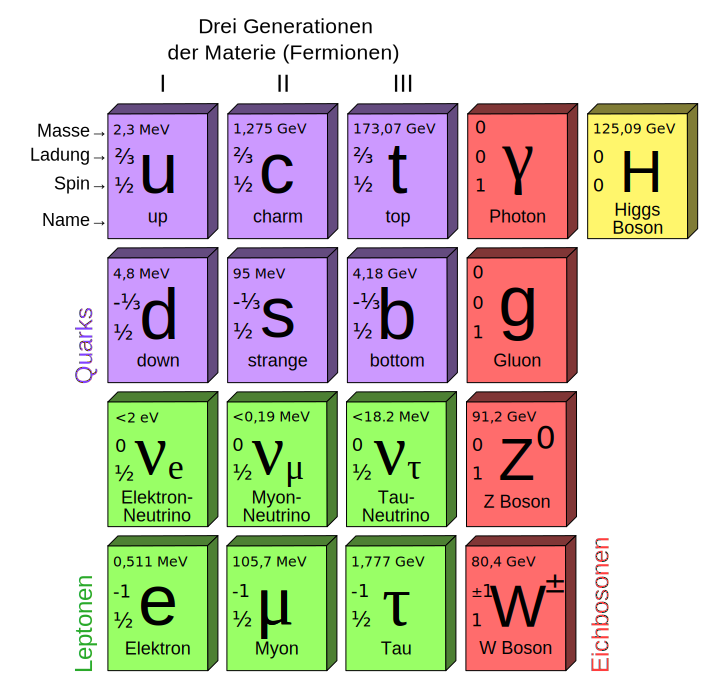
\includegraphics[width=5.5cm]{img/standardmodel}
			\caption*{Standardmodell\cite{standardmodel}}
		\end{figure}
	\end{column}
	\begin{column}{0.48\textwidth}
		$Z^0$-Boson:
		\begin{itemize}
			\item Lebensdauer $\tau\approx\SI{3e-25}{s}$
			\item Masse $M=\SI{91.2}{GeV}$
			\item ungeladen
			\item eigenes Antiteilchen
		\end{itemize}
	\end{column}
	\note[item]{Antiteilchen invers}
	\note[item]{Masse steigt mit Generation}
	\note[item]{Lebensdauer sehr sehr kurz}
	\note[item]{Masse (Reichweite)}
	\note[item]{ungleaden/neutral}
	\note[item]{Boson also Spin 1, außer Higgs}
	\note[item]{Schwache Wechselwirkung}
	\note[item]{Bestätigung der 3 Neutrinogenerationen}
\end{columns}

\end{iframe}

%\note[itemize]{
	%\item lila(Quarks), grün(Leptonen), rot(Eichbosonen), gelb(Higgs)
	%\item Generationen, Fermion , s=1/2
	%\item Boson s=1
	%\item Ladung Fermionen 2/3 -1/3 0 1  Bosonen 0 außer W \pm 1
	%\item Antiteilchen invers
	%\item
	%\item Masse steigt mit Generation
	%\item schwache WW
	%\item W+- => elek. Teilchen WW (beta Zerfall)
	%\item Z0 => auch neutral Teilchen WW (Neutrino)
%}

\subsection{Elektroschwache Vereinheitlichung}

\begin{iframe}


	\framesubtitle{Austauschteilchen}
	\begin{itemize}
		%\pause
		\item Photon $\rightarrow$ elektromagnetische Wechselwirkung
		%\pause
		\item W-, Z-Boson $\rightarrow$ schwache Wechselwirkung
		%\pause
		\item Gluon $\rightarrow$ starke Wechselwirkung
			\end{itemize}

\note[item]{Warum? Weil Divergenzen in höherer Ordnung/Energien auftreten } %TODO mehr
\note[item]{Vereint QED mit schwacher WW.}
\note[item]{ Kräfte durch Austauschteilchen}
\note[item] { Photon elektro magn. beispielweise Elektron-Elektron-Streuung, Rutherford Streuung}
\note[item]{W,Z bsplw. Beta-Zerfall, Elektron-Positron-Streuung (Energieabhänig)}
\note[item]{Gluon Kernzusammenhalt,Farbladung,8 (n-p-Anziehung), Quarkanziehung}

\note[item]{Nur durch Z-Boson lässt sich Neutrino-Neutrino-WW erklären, da sie nicht elektrisch sind.}

%\note[item]{ Allg. Grund + Was es ist.} %TODO:w

%\note[item] {?schwere Austauschteilchen => geringe Stärke der WW. (Graviton schwerer als Higgs)?} %TODO
%\note[item] {(experimentelle Bestimmung)}
%\note[item] {(Higgs)}
\end{iframe}

\begin{iframe}
	\framesubtitle{Schwacher Isospin}
	\begin{figure}
		\includegraphics[height=5cm]{img/isospin}
		\caption*{Schwacher Isospin\cite{povh}}
	\end{figure}
\note[item]{ Einführung von schwachem Isospin, analogon zu starkem Isospin}
	\note[item]{ Chiralität Index R/L formal: Zerlegung von Dirac-Spinoren in orthogonale Zustände die unter Paritätsoperationen ineinander übergehen. Eigenzustände $\pm1$}
	\note[item]{ Rechtshändige $e,\mu,\tau$ Singulett Zustand.}
		\note[item]{ Chiralität (l/r), Spinor Symmetrie}
	\note[item]{ Rechtshändige  Neutrinos $T_3=z=0$, keine WW, Auftreten in Natur unbekannt }
	\note[item]{ Der ' bedeuted != Masseneigenzustände, sondern Quarkmisch-Matrix CKM }

	\note[item]{$T_3$ Werte Bereich analog zu anderen Spins}
	\note[item]{ $z_f$ beschreibt Ladung }
\note[item] {invers für Antiteilchen: rechshändige Fermionen (linkshändige Antifermionen) Singulettt ($T=0=T_3$)}
	\note[item]{ Umwandung durch Absorption von $W^\pm$-Boson innerhalb Multiplett (darin Ladungsdifferenz = 1)}
\end{iframe}
	%\item ?was bedeutet der ' (Cabibbo-Rotation)? %TODO

\begin{iframe}
	\framesubtitle{Schwacher Isospin}
	\begin{columns}
		\begin{column}{0.48\textwidth}

			\begin{overprint}
				\onslide<1>\begin{figure}\includegraphics[height=4.5cm]{img/betadecay_old}\caption*{$\beta^-$-Zerfall\cite{beta}}\end{figure}
				\onslide<2>\begin{figure}\includegraphics[height=4.5cm]{img/betadecay_old}
\caption*{$\beta^-$-Zerfall\cite{beta}}\end{figure}
				\onslide<3>\begin{figure}\includegraphics[height=4.5cm]{img/betadecay}
\caption*{$\beta^-$-Zerfall\cite{beta}}\end{figure}
				\onslide<4>\begin{figure}\includegraphics[height=4.5cm]{img/kaondecay}
\caption*{$K^+$-Zerfall\cite{beta}}\end{figure}
				\onslide<5>\begin{figure}\includegraphics[height=4.5cm]{img/kaondecay}
\caption*{$K^+$-Zerfall\cite{beta}}\end{figure}
	\end{overprint}
	\end{column}
		\begin{column}{0.48\textwidth}

	\begin{itemize}
		\pause
		\item $T_3$ soll erhalten bleiben
		\pause
		\item $W^-$: $T_3=-1$
		\pause
		\item $W^+$: $T_3=1$
		\pause
		\item $W^0$: ($T=1,T_3=0$)
		\item $B^0$: ($T=0,T_3=0$)
	\end{itemize}
		\end{column}
	\end{columns}
	\only<1> {
	\note[item]{ Bekannt aus schwacher WW }
	\note[item]{ d$\rightarrow$u + $W^-$ }
	}
	\only<2> {
	\note[item]{$T_3$ Erhaltungsgröße}
	}
	\only<3> {
	\note[item]{$T_3$ in Graphik}
	\note[item]{$W^-$ muss -1 sein}
	%\note[item] {T: d(-1/2)=W(?)+u(1/2)}
	%\note[item] {T: W(?)=e(-1/2)+$\nu$(-1/2)}
	}
	\only<4> {
	\note[item]{ analog $\beta^+$-Zerfall: u$\rightarrow$d + $W^+$ }
	\note[item]{ Hier Kaon-Zerfall }
	}
	\only<5> {
	\note[item]{ Analog zu 1/2x1/2 Gekoppelten Spins}
	\note[item]{Tripplett und Singulett Zustände}
	\note[item] {$B^0$ postuliert}
	\note[item] {Mehr zum Beta-Zerfall nächste Woche (+Paritätsverletzung)}
	}
	%\note[item] {?Wieso T=1?} %TODO
\end{iframe}

\begin{iframe}
	\begin{itemize}
	\item Photon und $Z^0$ als orthogonale Linearkombination von $B^0$ und $W^0$:
		\begin{align*}
		 \ket{\gamma} &= +\cos{\theta_\text{W}} \ket{B^0} + \sin{\theta_\text{W}} \ket{W^0}	\\
		\ket{Z^0} &= -\sin{\theta_\text{W}} \ket{B^0} + \cos{\theta_\text{W}} \ket{W^0}
		\end{align*}
		\pause
	\item Weinbergwinkel:
		\begin{equation*}
		\cos{\theta_\text{W}}=\frac{M_\text{W}}{M_\text{Z}} \approx 0.88
		\end{equation*}
	\pause
		\item Gekoppelte Ladungen:
		\begin{equation*}
		e = g \cdot sin{\theta_\text{W}}
		\end{equation*}
	\end{itemize}
	\only<1> {
	\note[item]{ Drehung um Weinberg-Winkel/elektroschwachen Mischungswinkel , Naturkonstante}
	\note[item] {spontane Symmetriebrechung, diagonaliesierung der Massematrix führt zu diesen.}
	\note[item] {orthogonal + linear Kombination}
	}
	\only<2> {
	\note[item] {experimentelle Bestimmung, später mehr}
	\note[item] {Einziger Freier Parameter der Theorie.}
	\note[item] {Masse für $Z^0$ leichter zu Bestimmen, da W-Boson in Neutrino zerfällt. => bestimmung über fehlenden Transversalimpuls}
	}
	\only<3> {
	\note[item] {schwache Ladung g (Analogon zu e) aus schwache WW. aus QFT}
	\note[item] { beschreibbar durch elektrische und schwache Ladung}
	\note[item] {Umformung zu e/g  und M/M}
	}
\end{iframe}

%\subsection{Zerfallsbreite}

\section{Experimentelle Untersuchung}
\subsection{Erzeugung}

\begin{iframe}
	\begin{columns}
		\begin{column}{0.48\textwidth}
			\begin{figure}
				\feynmandiagram[large,horizontal=a to b] {
					i1 -- [fermion,edge label=\(e^-\)] a -- [fermion,edge label=\(e^+\)] i2,
					a -- [boson,edge label=\(\gamma\)] b,
					f1 -- [fermion,edge label'=\(\overline f\)] b -- [fermion,edge label'=\(f\)] f2,
				};
				\caption*{$e^+e^$-Vernichtung über $\gamma$ \cite{perkins}}
			\end{figure}
		\end{column}
		\begin{column}{0.48\textwidth}
			\begin{figure}
				\feynmandiagram[large,horizontal=a to b] {
					i1 -- [fermion,edge label=\(e^-\)] a -- [fermion,edge label=\(e^+\)] i2,
					a -- [boson,edge label=\(Z^0\)] b,
					f1 -- [fermion,edge label'=\(\overline f\)] b -- [fermion,edge label'=\(f\)] f2,
				};
				\caption*{$e^+e^$-Vernichtung über $Z^0$ \cite{perkins}}
			\end{figure}
		\end{column}
	\end{columns}
\end{iframe}

\note[itemize] {
	\item W/Z-Boson durch Antilepton+Lepton/AntiQuark+Quark Reaktion
	\item kollidierende Teilchenstrahlen
	\item feynman diagram
	\item Zeit nach rechts
	\item Antiteilchen Zeitlich invers (Aus Dirac-Gleichung (Schrödinger gleichung mit eingesetzter Impuls/Energie Relation wirkt auf vier komponentigen Dirac Spinor) ergeben sich positive und negative Lösungen für die Energie) (bzw. Klein Gordon Gleichung (entkoppelt)) nach Stückelberg-Feynman-Interpretation, bsplw. E-Feld $e^-$ vs $e^+$ mit anderer Richtung ist gleich. (Dirac sagte Antiteilchen vorher/definierte, wobei negative Energien besetzt sind und Löcher sich ausbreiten basierend auf Pauli-Ausschlussprinzip, da Bosonen nicht gehorchen => reverse Zeit Interpretation)
	\item über $\gamma $oder $Z$ zu Fermion und Antifermion paar.
	\item bei passender Energie\ approx $M_Z$  dominiert $Z^0$, aus QFT+Feynmanregeln
}

\begin{iframe}
	\begin{itemize}
		\item Schwerpunktsenergie $\sqrt{s} = 2E_e \geq M_\text{Z}c^2 \approx \SI{91.6}{GeV}$
		\pause
		\item $pp$-Kollision: $u + \overline{u} \rightarrow Z^0 $ benötigt $\sqrt{s} \gtrapprox \SI{600}{GeV}$ pro Proton
		\pause
		\item $e^+ + e^- \rightarrow W^+ + W^-$ benötigt $\sqrt{s} \geq 2M_\text{W}c^2 \approx \SI{160.8}{GeV}$
	\end{itemize}
	\note[item]{ 1989 am Stanford Linear Collider und LEP}
	\note[item]{Energie muss in Quarks enthalten sein $\rightarrow$ sehr viel mehr Energie auf Protonen (analog mit d) => e-e+ Kollision einfacher}
	\note[item]{ 1996 am LEP, 50 $\rightarrow$ 86 $\rightarrow$  \SI{104.6}{GeV}}
\end{iframe}

\begin{iframe}
	\framesubtitle{Luminosität}
	\begin{equation*}
		\dot{N}_f = \sigma_f \mathcal{L}
	\end{equation*}
	\begin{figure}
		\includegraphics[height=3.5cm]{img/bhabha}
		\caption*{Bhabha Streuung \cite{huz0}}
	\end{figure}
	\note[item] {Gibt Events pro Zeit Detektion pro Wirkungsquerschnitt an.}
	\note[item]{Luminosität hängt von Beschleuniger ab}
	\note[item]{sigma ist gesucht}
	\note[item]{N sind Anzahl Teilchen be REaktion}
	\note[item]{eig. noch Fehler korrektur mit Akzeptanzraten und Effizienzen}
	\note[item]{Wirkungsquerschnitt für Bhabha-Streuung ee -> ee reine QED ziemlich genau bekannt (Kamera am detektor?)}
\end{iframe}


\begin{iframe}
\framesubtitle{Einfluss durch Gezeiten}
\begin{figure}
		\includegraphics<1>[height=5cm]{img/gezeit}
		\includegraphics<2>[height=5cm]{img/tide}
		\only<1>{\caption*{LEP Ausdehunung\cite{cern}}}
		\only<2>{\caption*{Relative Strahlenergieänderung\cite{huz0}}}
	\end{figure}
	\note[item]{weiter Effekt}
	\note[item]{Energie schwankt im Tages verlauf}
	\note[item]{Resonante depolarisation} %TODO
	\note[item]{Größe primär relevant für Energie (+Synchrotron strahlung)}
\end{iframe}
\subsection{Nachweis}
\begin{iframe}
	\framesubtitle{Detektor}
\begin{figure}
		\includegraphics<1>[height=5cm]{img/skizze}
		\includegraphics<2>[height=5cm]{img/detektor}
		\caption*{L3 Detektor \cite{huz0}}
	\end{figure}
	\note[item]{Analog Vorlesung, Hadronen Jets}
	\note[item]{Masse/Ladung durch Felder+ Drifts mit Magnetfeld}
\end{iframe}
%TODO Detektor aufbau
\begin{iframe}
	\framesubtitle{1983 am CERN}
	\begin{figure}
		\includegraphics[width=6cm]{img/lego}
		\caption*{$q+\overline{q} \rightarrow Z^0 \rightarrow e^+ + e^-$ \cite{povh}}
	\end{figure}
\end{iframe}

\note[itemize] {
	\item Plane unten sind Kaloriemeterzellen
	\item Energie Summe $=$ Masse $Z^0$
	\item Beispiel Event einer Messung
	\item Winkel 180° => entgegen gesetzte Richtungen

	\item ?Woher sicher, dass $Z^0$ Zerfall?
}

%TODO andere GRaphiken für Jet+ee
\begin{iframe}
	\framesubtitle{1993 am LEP/CERN}
	\begin{figure}
		\includegraphics<1>[height=5cm]{img/hadron}
		\includegraphics<2>[height=5cm]{img/elektron}
		\includegraphics<3>[height=5cm]{img/muon}
		\only<1>{\caption*{$e^- +e^- \rightarrow Z^0 \rightarrow$ hadronische Jets \cite{huz0}}}
		\only<2>{\caption*{$e^- +e^- \rightarrow Z^0 \rightarrow e^+ + e^-$ \cite{huz0}}}
		\only<3>{\caption*{$e^- +e^- \rightarrow Z^0 \rightarrow \mu^+ + \mu^-$ \cite{huz0}}}
	\end{figure}
	\note[item]{Balken sind die Energien die Kaloriemeter messen}
	\note[item]{ L3 detector LEP}
	\note[item]{ Beispiel Muon}
	\note[item]{ Winkel 180° => entgegen gesetzte Richtungen}
	\note[item]{?Woher sicher, dass $Z^0$ Zerfall?}
\end{iframe}

\subsection{Eigenschaften}
\begin{iframe}
	\framesubtitle{Experimentelle Bestimmung}
	\begin{itemize}
		\item Messung: %TODO Graphik!!
		\begin{itemize}
			\item $M_Z = \SI{91.188+-0.002}{GeV/c^2}$
			\item $\Gamma_Z = \SI{2.495+-0.002}{GeV}$
		\end{itemize}
		\pause
		\item Zerfall:
		\begin{align*}
			Z^0 \rightarrow & e^+ + e^- & \SI{3.363+-0.004}{\%} \\
			& \mu^+ + \mu^- & \SI{3.366+-0.007}{\%} \\
			& \tau^+ + \tau^- & \SI{3.370+-0.008}{\%} \\
			& \nu_{e,\mu,\tau}^+ + \overline{\nu}_{e,\mu,\tau} & \SI{20+-0.06}{\%} \\
			& \text{Hadronen} & \SI{69.91+-0.06}{\%} \\
		\end{align*}
	\end{itemize}
\note[item]{Über Wirkungsquerschnitt? src [PD12]}
\note[item]{}
\note[item]{Hadronen (idR. Anti+Quark) nicht unterscheidbar}
\note[item]{Anti+Neutrino schwer detektierbar => \% über $\Gamma_\text{tot}$}
\note[item]{totale Breite = alle Zerfälle Anti+Fermion???}
%\note[item]{$Z^0$ nicht nur ungeladenes $W$-Boson, da }
\end{iframe}

\subsection{Neutrinogenerationen}

\begin{iframe}
	\framesubtitle{Wirkungsquerschnitt}
	\begin{columns}
		\begin{column}{0.48\textwidth}
			\begin{equation*}
				\sigma_f =  \frac{12 \pi \cdot \Gamma_f\cdot \Gamma_e}{(s-M_Z^2)^2 + M_Z^2\Gamma_Z^2}
			\end{equation*}
		\end{column}
		\begin{column}{0.48\textwidth}
		\end{column}
	\end {columns}
	\begin{textblock*}{5cm}(7cm,3cm) % {block width} (coords)
				\begin{figure}
				\feynmandiagram[large,horizontal=a to b] {
					i1 -- [fermion,edge label=\(e^-\)] a -- [fermion,edge label=\(e^+\)] i2,
					a -- [boson,edge label=\(Z^0\)] b,
					f1 -- [fermion,edge label'=\(\overline f\)] b -- [fermion,edge label'=\(f\)] f2,
				};
			\end{figure}
		\end{textblock*}
\note[item]{Formel für $\sigma$ Breit-Wigner}
\note[item]{Einheiten $h$ und $c$ multiplizieren}
\note[item]{Abhängig von ...}
\note[item]{$\gamma$ unterdrückt}
\end{iframe}

\begin{iframe}
	\framesubtitle{Zerfallsbreite}
	\begin{align*}
		\action<+->{\Gamma_Z&=\sum_f \Gamma_{Z \rightarrow f\bar{f}}\\}
		\action<+->{&= \Gamma_\text{Had}  + \Gamma_\text{Lep}+ \Gamma_\nu\\}
		\action<+->{&= N_C \cdot2\cdot\Gamma_u + N_C\cdot 3\cdot \Gamma_d + 3\cdot\Gamma_e + 3\cdot\Gamma_\nu\\}
		\action<+->{&= 3 \cdot 2\cdot\SI{94.9}{MeV} + 3\cdot3\cdot \SI{122.4}{MeV}+ 3\cdot \SI{83.3}{MeV} + 3\cdot \SI{165.8}{MeV} \\} %TODO fix SI font
		\action<+->{&=\SI{2.42}{GeV}\\}
		\action<+->{&\xrightarrow[\text{korrektur}]{\text{Strahlungs-}}\SI{2.497}{GeV}\\}
	\end{align*}
\note[item]{$\Gamma_f=\frac{G_F M_Z^3}{24\sqrt{2}\pi}\cdot (1+(1-e|Q_f|\sin^2{\theta_W})^2)$}
\note[item]{$G_F$ Fermikonstante}
\note[item]{$Q_f$ Ladung des Fermions}
\note[item]{ Lep: $e^\pm$, $\mu^\pm$, $\tau^\pm$}
\note[item]{ Had: u,c= 2/3; d,s,b=-1/3}
\note[item]{ Neutrinos}
\note[item]{kein top-Quark weil nicht genug Energie aus $Z^0$ ($\approx \SI{175}{ GeV}$)}
\note[item]{Korrekturen aus QFT, höherer Ordungen, Strahlungskorrektur}
\note[item]{Passt mit Unsicherheiten zu Exp. (nicht auf Folie)}
\note[item]{$\Gamma_e/\Gamma_{tot}=3,37\%$ passt auch zu Exp.}
\end{iframe}

\begin{iframe}
	\begin{figure}
		\includegraphics[width=5.5cm]{img/neutrinogen}
		\caption*{Wirkungsquerschnitt $e^+e^-\rightarrow $Hadronen \cite{povh}}
	\end{figure}
	\note[item]{Cern Experiment}
	\note[item]{Schwerpunkt energie gegen Wirkungsquerschnitt}
	\note[item]{Ähnlich der Breit Wigner Funktion aber nicht passend symmetrisch durch Korrekturen höherer Ordnung udn Bremstrahlung durch $e^-$}
	\note[item]{Verschiedene Anzahl-Neutrinogenerationen-Kurven}
	\note[item]{3 Neutrinogenerationen $\rightarrow$ 3 Leptonen 3 Quarks Generationen}
\end{iframe}
%TODO Neutrino generationen


\section{Zusammenfassung}
%\subsection{Zusammenfassung}
\begin{frame}
	\frametitle{Zusammenfassung}
\begin{itemize}
	\item Schwache und Elektromagnetische Wechselwirkung lassen sich vereinheitlichen
	\item	Weinbergwinkel $\cos{\theta_\text{W}} \approx 0.88$
	\item Zerfallsbreite $\Gamma_Z \approx \SI{2.50}{GeV}$
	\item 3 Neutrinogenerationen
\end{itemize}
\note[item]{Weinbergwinkel Massenverhältniss W,Z Boson}
\note[item]{Zerfallsbreite aus QFT großer Erfolg in Übereinstimmung mit Experiment}
\note[item] { Bestätigung, dass es 3 Neutrinogenerationen gibt}
	\note[item] {Weiterfüherend Große Vereinheitlichung Analog ab \SI{e16}{GeV} => keine Differenzierung Fermionen,Quarks und Leptonen. (Astrovorträge, Universumentwicklungröhre)}
\note[item] {Noch Weiterfüherend Quantengravitation kombiniert mit GUT}
%TODO Daten für relevante Events wdh.
\end{frame}


\begin{frame}[allowframebreaks]
	\frametitle{Quellen}
	\renewcommand*{\bibfont}{\small}
	\printbibliography[heading=none]
\end{frame}
\note[itemize] {\item Masterclasses Atlas ist qualitativ gut}

\begin{frame}
	\begin{block}{}
		\centering
		Vielen Dank für eure Aufmerksamkeit!
	\end{block}

	\begin{block}{}
		\centering
		Fragen?
	\end{block}

\end{frame}

\end{document}
